\documentclass[11pt,a4paper]{scrartcl}

\usepackage{fullpage}

%\usepackage[ngerman]{babel}
\usepackage[utf8]{inputenc}
\usepackage{graphicx}

\usepackage{amsmath}
\usepackage{amsfonts}
\usepackage{amsthm}
%\usepackage{mathtools}

\usepackage{listings}

%%%%% COMMANDS

\newcommand{\FT}{\mathcal{F}}
\newcommand{\T}{\mathrm{T}}
\newcommand{\IFT}{\mathcal{F}^{-1}}
\newcommand{\conv}{\ast}
\newcommand{\defined}{\coloneqq}
\newcommand{\IR}{\mathbb{R}}
\newcommand{\IZ}{\mathbb{Z}}
\newcommand{\map}{\rightarrow}


\newtheorem*{theorem}{Theorem}

\renewcommand{\thesubsection}{\alph{subsection})}

\begin{document}

\title{Artificial Intelligence Exercise 2}
\author{Markus Döring, 3153320}
\maketitle

\section{Search Algorithms}
\subsection{Tree Traversal}
% \begin{figure}[ht]
%  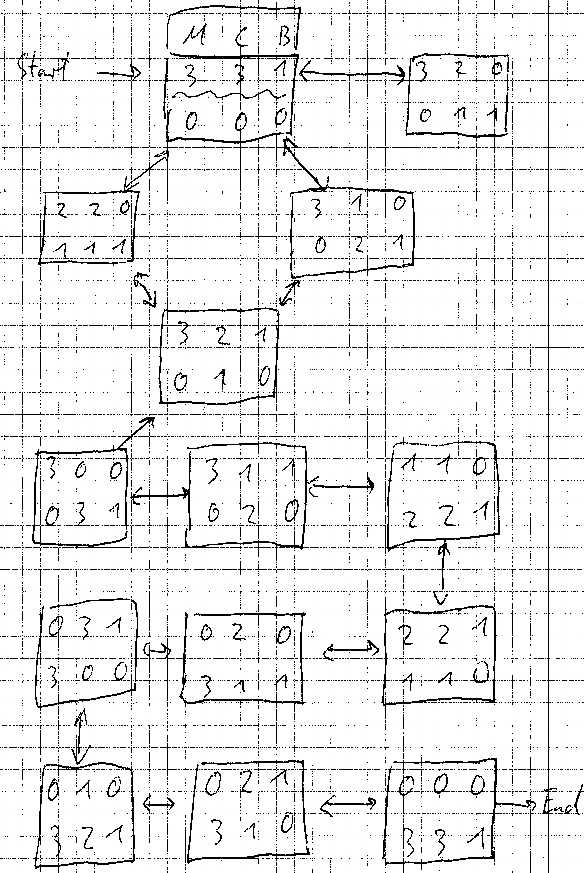
\includegraphics[width=.65\linewidth]{missionaries_cropped.jpg}
%  \caption{The state space graph of the missionary-cannibal-boat problem. The columns denote the objects (M, C, B), the rows the location (side of the river). It turns out that most possible states are not allowed by the problem statement.}
% \end{figure}

\subsection{Infinite Trees}

If the depth of a search tree is infinite, then depth-first search is in general 
not complete - it can get stuck in one infinite branch while the goal state is 
in another one. Breadth-First search is compelete for trees with infinite depth, 
because all nodes of one layer are visited before the algorithm advances to the 
next layer. Trees with infinite width could be a problem for breadth-first search, 
but such trees would turn out much more problematic in other ways, namely memory 
usage.

\section{Water-Jug Problem}

\subsection{Problem}
We represent the state with a vector $s = (x,y)^T\in\IR^2$, with entries $x,y$ standing 
for the amount of water in each jug, in liters. The initial state would therefore 
be $(0,0)^T$, and the target state $(0,4)^T$. Path costs can be chosen constant 
as $c=1$. An action $f:\ \IR^2\map\IR^2,$ is valid if

\begin{itemize}
\item $f(x,y) = (0,y)^T$ or
\item $f(x,y) = (x,0)^T$ or 
\item $f(x,y) = (\min(\{3, x+y\}), y-\min(\{3-x,y\}))^T$ or
\item $f(x,y) = (x-\min(\{5-y,x\}), \min(\{5,x+y\}))^T$.
\end{itemize}

\subsection{State-Space Graph}
% \begin{figure}[ht]
%  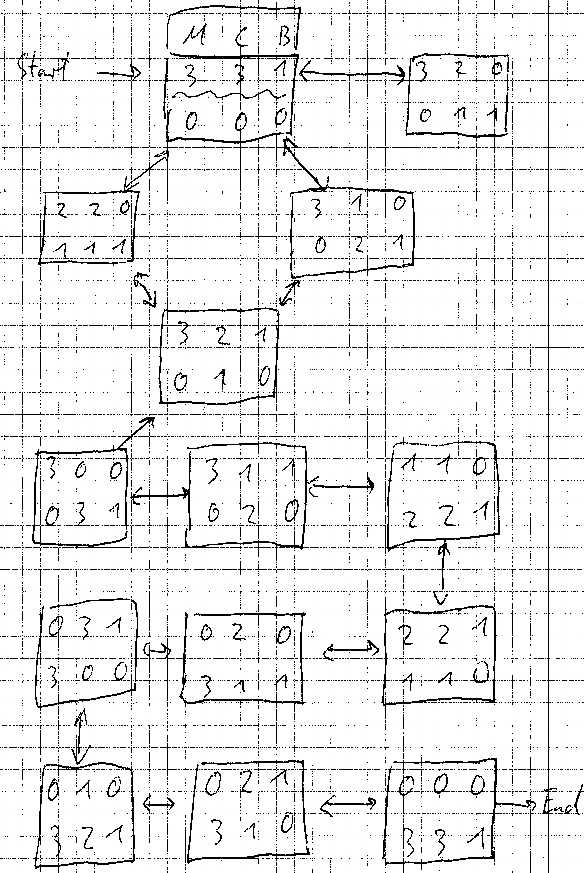
\includegraphics[width=.65\linewidth]{missionaries_cropped.jpg}
%  \caption{The state space graph of the missionary-cannibal-boat problem. The columns denote the objects (M, C, B), the rows the location (side of the river). It turns out that most possible states are not allowed by the problem statement.}
% \end{figure}

\subsection{}
Obvious.

\section{Missionaries and Cannibals}

See the python script \emph{mcb.py}. 

\section{Optimality of $A^*$}

\begin{theorem}
Let $h$ be an admissible heuristic function, that is for all nodes $n$ and for the 
true cost function $h^*$ 
\begin{equation}\label{eq:adm}
h(n)\leq h^*(n)
\end{equation}
holds. Then the $A^*$ algorithm is optimal on the search tree $T$.
\end{theorem}
\begin{proof}
Let $f(n) = g(n) + h(n)$ denote the desirability function that $A^*$ tries to 
minimize. The function $g$ gives the true cost up to node $n$, and $h$ is the 
heuristic. Let $m,n$ be two states on paths $P_m, P_n$ to a goal state, and let 
$P_m$ be more expensive than $P_n$. Let $m$ be adjacent to the goal state on path 
$P_m$. Then $A^*$ is optimal if and only if node $n$ is erxpanded before node $m$.  

We prove the theorem indirectly. Assume node $m$ gets expanded before node $n$. 
This implies that $f(n)>f(m)\Leftrightarrow g(n) + h(n) > g(m) + h(m)$. Path $P_n$
is shorter than path $P_m$, and therefore 
\begin{equation}
g(n)+h^*(n) < g(m) + h^*(m) \stackrel{\text{Eq. \ref{eq:adm}}}{\leq} g(m) + h(m) < g(n) + h(n), 
\end{equation}
which contradicts the admissability of $h$. Therefore, $m$ does not get expanded before any node on 
path $P_n$, and $A^*$ finds the optimal solution. 
\end{proof}
%\newpage
%\appendix
%\lstinputlisting[language=python]{ia_05_01.py}
%\newpage
%\lstinputlisting[language=python]{ia_05_02.py}
\end{document}
